%
% File: chap01.tex
% Author: Victor F. Brena-Medina
% Description: Introduction chapter where the biology goes.
%
\let\textcircled=\pgftextcircled
\chapter{Modelling the effect of actuator-like behavior in dielectric elastomer generators}
\label{chap:1}

\initial{T}his chapter is based on the paper ''Modelling the effect of actuator-like behavior in dielectric elastomer generators``, published in the Volume 107 of Applied Physics Letters in 2015.

Dielectric elastomers have a dual behavior, able to convert electrical energy into mechanical if charged electrostatically and to convert mechanical to electrical energy if stretched and relaxed in a cycle that exploits its capacitance change. During such energy harvesting cycles, the material needs an electrical energy bias to be able to convert mechanical work into electrical energy, which produces an actuator behavior on the DEG that results in losses and decreases its performance. In this paper, we investigate this actuation behavior and its effect on energy harvesting in DEGs. We compare two different charging methods and show that a constant voltage method can increase the net energy harvested by 5 times, despite the unwanted actuation effect.




%=======
\section{Introduction}
\label{sec:intro}

When designing and modelling energy harvesting cycles for DEGs, there are two possible scenarios to take into account: position-based or force-based cycling. Position-based cycling corresponds to most mechanical systems, such as cranked mechanisms, where the strain cycle is fixed. Force based cycling more accurately emulates natural phenomena, such as waves and wind gusts, from which we may wish to harvest renewable energy. In these phenomena, a pressure or force variation acts against the material and strain is not mechanically constrained. 

Many previous studies have designed harvesting cycles\cite{RN85,RN629,Shian2014OptimizingGenerators} but none has taken into account the actuation-like behavior induced when the material is charged. In a position based cycle, that yields a softening of the material, reducing the force induced by the membrane elasticity, as can be noticed in experiments reported in \cite{RN1}, where after charging it is possible to notice a drop in the force measurements across the DEG.
When dealing with force-based scenarios, the actuator like behaviour corresponds to an increase in stretch due to the charges added and will happen differently depending on how the charging is controlled.

Since energy harvested is proportional to the bias electrical energy input during charging, energy harvesting capabilities are thought to increase with the use of higher electric fields. On the other hand, as the electric field is increased towards material limits, the charge-induced actuation will be an increasingly important issue, which must be taken into account in any realistic energy harvesting cycle.

This chapter seeks both to report the phenomenon of charge-induced actuation, focusing on force-based scenarios and to understand how to deal with it, through comparisons of energy input, conversion and losses. 

\section{Methods}
\label{sec:methods}
To evaluate the actuation after the charging phase, we compare two different methods to move from the stretched and uncharged state to the stretched and charged state. Both are illustrated in Figure 1, and involve transition from state 2 (stretched and uncharged) to equilibrium at state 3 (stretched and charged with bias voltage) via different intermediate states. The first method (mode A), instantaneously injects sufficient charge at state 2 to elevate the bias electric field to state 2.5\textquotesingle.  The electrical supply is then disconnected. The DEG then undergoes actuation as a result of this electric field, moving it to state 3.  In the second method (mode B), a voltage is instantaneously applied at state 2 to raise the electric field to state 2.5\textquotedbl. The DEG then undergoes actuation as a result of this constant voltage. Electric field and strain both increase until state 3 is reached.  The applied voltage is chosen such that state 3 exactly matches that for mode A. Having the same state for both methods guarantees that all remaining characteristics of the cycle are identical. 

\begin{figure}
   \begin{center}
   \begin{tabular}{c} %% tabular useful for creating an array of images 
   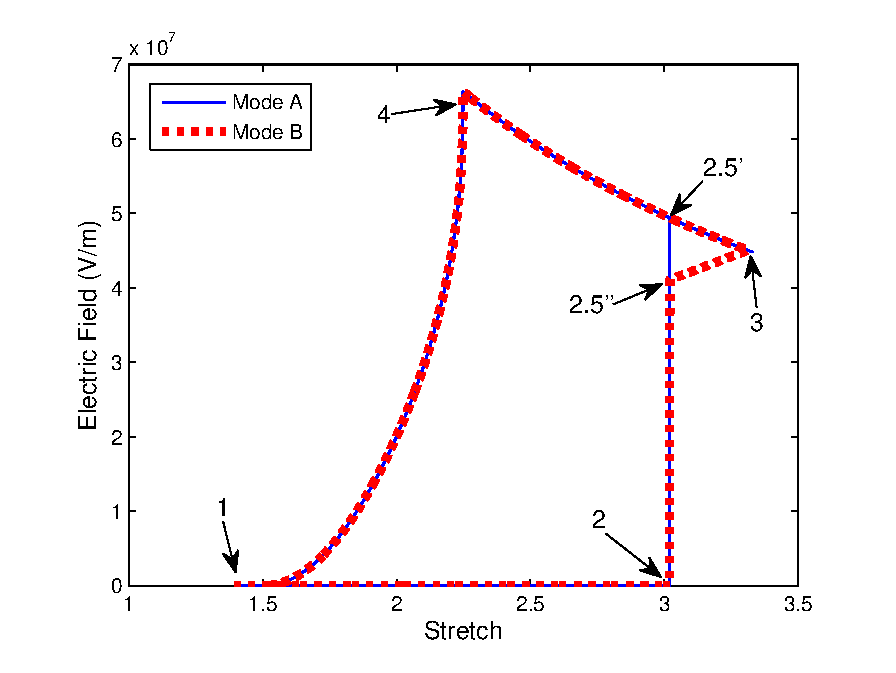
\includegraphics[scale=0.8]{fig02/Fig1.eps}
   \end{tabular}
   \end{center}
   \caption[example] 
%>>>> use \label inside caption to get Fig. number with \ref{}
   { \label{fig:Cycle SxE} 
Electric field versus stretch ratio of the DEG, for both charging modes.}
\end{figure}


   \begin{figure}[h]
   \begin{center}
   \begin{tabular}{c} %% tabular useful for creating an array of images 
   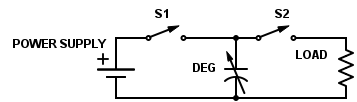
\includegraphics[scale=1.0]{fig02/circuit.png}
   \end{tabular}
   \end{center}
   \caption[example] 
%>>>> use \label inside caption to get Fig. number with \ref{}
   { \label{fig:circuit} 
DEG circuit: S1 allows the DEG to charge under constant voltage, while S2 discharges the DEG through a constant load.}
   \end{figure} 
 

	In order to evaluate the electrical and viscous losses for both charging modes we impose a sinusoidal mechanical forcing at 1Hz. This simulates a real scenario such as wave energy harvesting or a human walking. We compare numerically the two charging modes and explore their actuation characteristics. The DEG model assumes uniaxial stretching of the membrane, considering the material width to be constant (i.e. pure shear). Material parameters for the simulation were taken from an approximation of the shear modulus of 3M VHB 4910 from Ogden model parameters derived by Wissler and Mazza\cite{RN46}. DEG sample considered had initial area of 0.02m$^2$ and was 0.1mm thick, with initial capacitance of 8.3nF. The charging/discharging circuit is shown in Figure 2. At the start of the cycle, both S1 and S2 are open. At the end of the stretching phase, S1 is closed and the material is allowed to charge.  For mode A, S1 is reopened as soon as state 2.5\textquotesingle{} is reached.  For mode B, S1 is reopened when equilibrium state 3 is reached. At the end of the relaxing phase (state 4) S2 is closed to allow the discharge of the energy output. 
 
   \begin{figure}[h]
   \begin{center}
   \begin{tabular}{c} %% tabular useful for creating an array of images 
   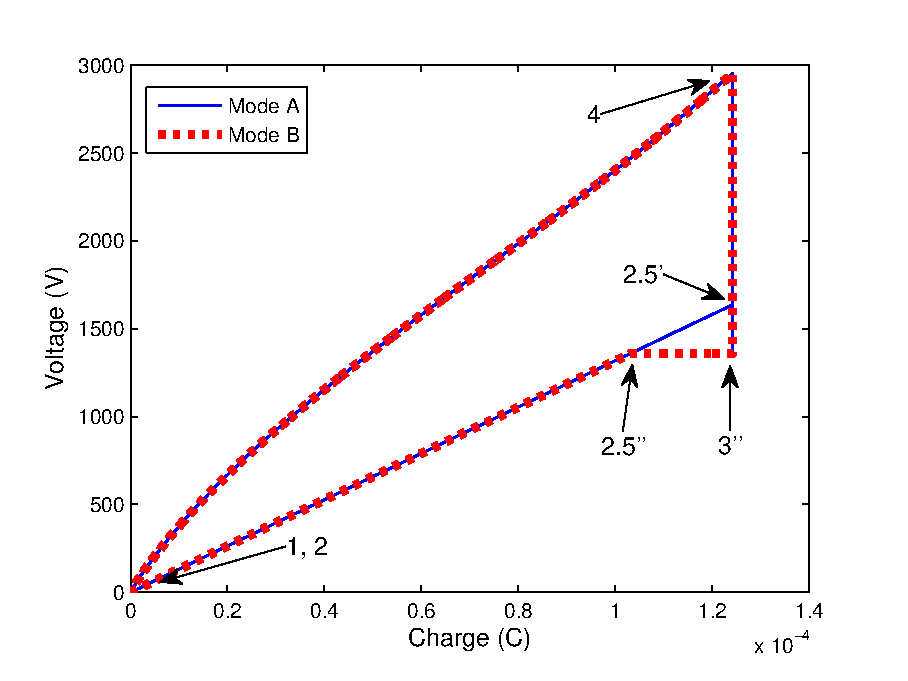
\includegraphics[scale=0.8]{fig02/Fig3.eps}
   \end{tabular}
   \end{center}
   \caption[example] 
%>>>> use \label inside caption to get Fig. number with \ref{}
   { \label{fig:Cycle QxV} 
Voltage versus charge plot for the DEG.}
   \end{figure}  
 

In order to couple the charging modes with the electromechanical model of a DEG, a common method is to consider equilibrium states of a harvesting cycle\cite{Shian2014OptimizingGenerators,RN73,RN32}. Here we developed a simulation model based on Graf et al\cite{RN73}, applied to a uniaxially deformed material. The deformation of the DEG, x, evolves according to
\begin{equation} \label{eq:1}
m \ddot{x} = F_x- d_v \dot{x} -  \frac{B}{x} \left( G \frac{\lambda_x^4-1}{\lambda_x^2} +\sigma_z \right)
\end{equation}


where $m$ is the equivalent mass, $F_x$ is the applied force, $d_v$ is the damping coefficient, $B$ is the total volume, $G$ is the shear modulus (Neo-Hookean model) and $λ_x$ is the stretch ratio. The applied stress, $\sigma_z$, is given by
\begin{equation} \label{eq:2}
\sigma_z = -e_r e_0 \left(\frac{V}{z}\right)^2 = -e_r e_0 \left(\frac{V}{z_0} \right)^2 \lambda_x^2
\end{equation}


where $e$ is the material permittivity, $V$ the applied voltage, $z_0$ the initial thickness. The charge stored, $Q$, and the capacitance, $C$, are included via the standard relationship
\begin{equation} \label{eq:3}
V=Q/C
\end{equation}

To find equilibria, we can substitute \ref{eq:2} into \ref{eq:1}, yielding

\begin{equation} \label{eq:4}
F_x =   \frac{B}{x_0^2}  \left(G-e_r e_0 \left(\frac{V}{z_0} \right)^2 \right)x-B G \frac{x_0^2}{x^3}  
\end{equation}

which, with \ref{eq:3}, allows us to prescribe independently any two of the four states ($x$,$V$,$Q$,$F$) and determine the remaining ones.

\section{Results and discussion}
\label{sec:results}

\subsection{Charging - Electrical point of view}
\label{subsec:charging}
Considering the viscous nature of most DEs, it is reasonable to assume that the charging and discharging processes occur much faster than the mechanical deformations due to the electrostatic forces, specially since in its manufacture, low resistance electrodes are an important aspect. The consequences of such behavior is shown in Figure \ref{fig:Cycle QxV}, which allows us to visualize mode A: after state 2, charging occurs under constant capacitance, leading to the unstable state 2.5\textquotesingle, which then relaxes and approaches equilibrium at stage 3 again.

   \begin{figure}[htb]
   \begin{center}
   \begin{tabular}{c} %% tabular useful for creating an array of images 
   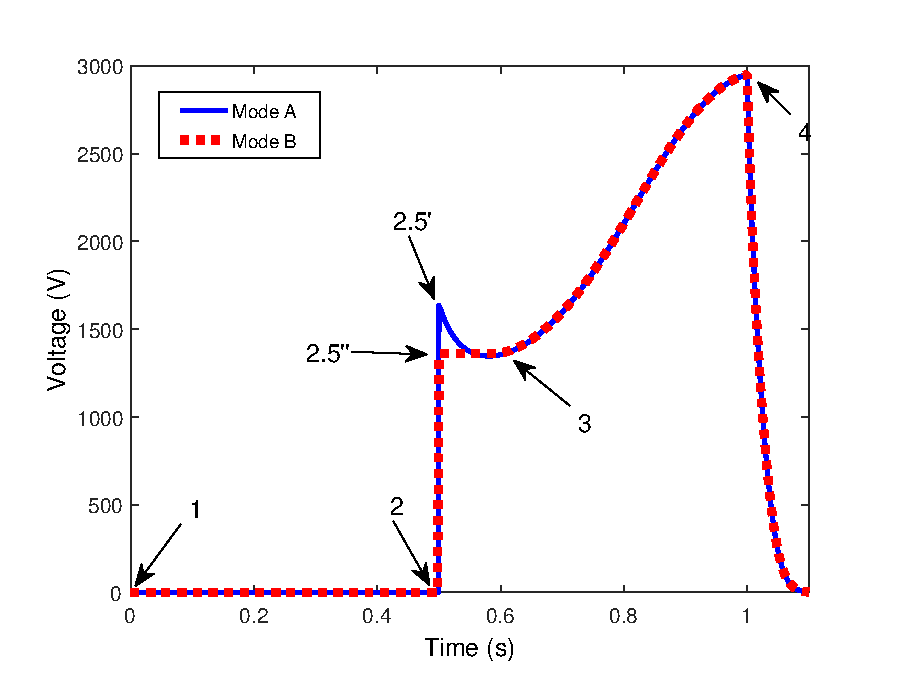
\includegraphics[scale=0.8]{fig02/Fig4_unit.eps}
   \end{tabular}
   \end{center}
   \caption[example] 
%>>>> use \label inside caption to get Fig. number with \ref{}
   { \label{fig:Cycle txV} 
Voltage of the DEG as a function of time.}
   \end{figure}  



In Figure \ref{fig:Cycle txV}, we show the evolution of voltage as a function of time, for both charging modes, as the DEG undergoes 1 Hz sinusoidal forcing. State 2 occurs just before the bias voltage is applied, while state 3 takes place when both the curves match before transition to state 4 (around 0.58 s). 

Note that although the curves approximately converge to the equilibrium state 3, they do not match perfectly at this point, since the model we simulate is dynamic, and it is not possible to reach an equilibrium (in a smooth system) in finite time. However, the two trajectories do converge quickly, and then proceed to the same state 4 prior to discharge, outputting the same amount of energy. Notice that time taken for the trajectories to converge depends on the material viscosity and the magnitude and frequency of the electrical and mechanical loads applied.

When charging a constant value capacitor to a voltage $V$, in order to store a charge $Q$ it is necessary to expend an amount of energy VQ, although only $VQ/2$ is stored. Hence, when charging with constant capacitance, there is an implicit loss of 50\% of the electric energy input. Wang et al\cite{RN1} suggest that to guarantee that energy will be harvested in a cycle it is necessary that the capacitance of the charging state should be at least twice the capacitance of the discharging state.
On the other hand, when charging with constant voltage, we have a change in energy $U_e$ of
\begin{equation}
	U_e= \int_{Q_1}^{Q_2}V dq=V(Q_2-Q_1)	
\end{equation}

Since half this energy is stored, as before, the other half is converted to mechanical work, as described for actuator behaviour by Carpi et al\cite{RN43}. 

From Figure \ref{fig:Cycle QxV} it is easy to see how high the losses can be while charging in mode A compared to mode B. In mode B, the charging can be divided into two phases: the first, to voltage $V_3$ and charge $Q_2.5$ ) and the second, under constant voltage, to voltage $V_3$ and charge $Q_3$. The area below the curves in Figure \ref{fig:Cycle QxV} shows the amount of energy expended in charging. The triangle between the points 2.5\textquotesingle, 2.5\textquotedbl and 3 corresponds to the extra work done in mode A.
We compare both charging energies, calculated by direct simulation, in table I. In order to have 85 mJ electric energy stored in state 3, it is necessary to input 190 mJ electric energy using mode A, but only 160 mJ using mode B (for the same stored energy). The electric energy dissipated in this process corresponds to the 50\% lost during capacitor charging, together with losses in the resistive elements (e.g. electrodes).

\subsection{Charging - Mechanical point of view}
\label{subsec:charging}

   \begin{figure}[htb]
   \begin{center}
   \begin{tabular}{c} %% tabular useful for creating an array of images 
   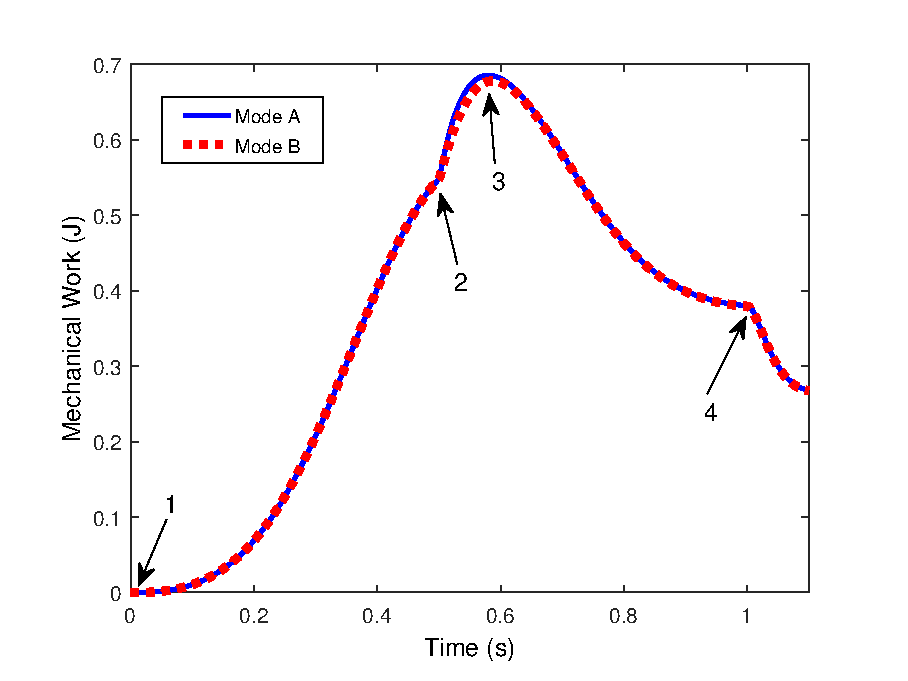
\includegraphics[scale=0.8]{fig02/Fig5_unit.eps}
   \end{tabular}
   \end{center}
   \caption[example] 
%>>>> use \label inside caption to get Fig. number with \ref{}
   { \label{fig:Cycle txW} 
External work done to the DEG as a function of time.}
   \end{figure}  

   \begin{figure}[htb]
   \begin{center}
   \begin{tabular}{c} %% tabular useful for creating an array of images 
   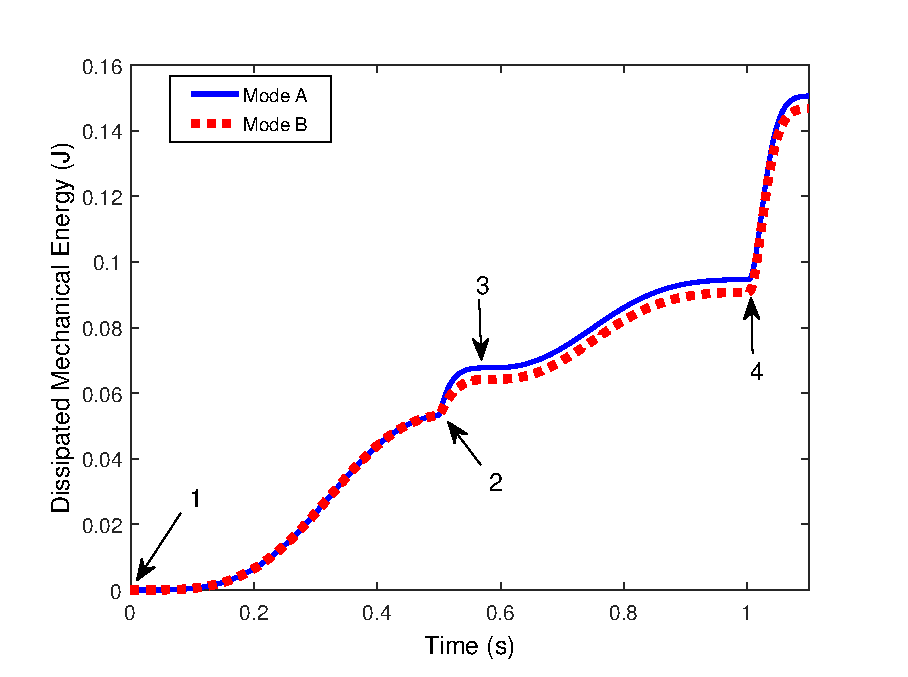
\includegraphics[scale=0.8]{fig02/Fig6_unit.eps}
   \end{tabular}
   \end{center}
   \caption[example] 
%>>>> use \label inside caption to get Fig. number with \ref{}
   { \label{fig:Cycle txW_loss} 
Viscous losses over time for both the charging methods applied on an energy harvesting cycle.}
   \end{figure}   

\begin{table}[htb]
\caption{Electrical energy balance during process 2-3 comparing charging modes A and B.} 
\label{tab:1}
\begin{center}       
\begin{tabular}{|l|l|l|l|}
\hline
\rule[-1ex]{0pt}{3.5ex}   & & Mode A & Mode B  \\
\hline
\rule[-1ex]{0pt}{3.5ex}  a & Electric Energy Input at 2.5 & 0.190 J	& 0.131 J\\
\hline
\rule[-1ex]{0pt}{3.5ex}  b & Electric Energy Input 2.5-3 &0 J & 0.029 J\\
\hline
\rule[-1ex]{0pt}{3.5ex}  c & Total Electric Energy input 2-3 (a+b)	&0.190 J&	0.160 J \\
\hline
\rule[-1ex]{0pt}{3.5ex}  d & Electric Energy Dissipated 2-3 &	(0.088) J&	(0.061) J\\
\hline 
\rule[-1ex]{0pt}{3.5ex}  e&	Actuation Energy (electrical to mechanical conversion) 2-3&	(0.017)J &(0.014) J\\
\hline 
\rule[-1ex]{0pt}{3.5ex}  f& Electric Energy Stored at 3 (c+d+e)	&0.085 J	&0.085 J\\
\hline 
\end{tabular}
\end{center}
\end{table}

		
\begin{table}[htb]
\caption{Mechanical energy balance during process  2-3 comparing charging modes A and B.} 
\label{tab:2}
\begin{center}       
\begin{tabular}{|l|l|l|l|}
\hline
\rule[-1ex]{0pt}{3.5ex}   & & Mode A & Mode B  \\
\hline
\rule[-1ex]{0pt}{3.5ex}  g&	External Mechanical Work 2-3	&0.138 J	&0.130J\\
\hline
\rule[-1ex]{0pt}{3.5ex}  h & Mechanical Energy Damped 2-3	&(0.014) J	&(0.011) J\\
\hline
\rule[-1ex]{0pt}{3.5ex}  i & Actuation Energy (electrical to mechanical conversion) 2-3	&0.017 J&	0.014 J \\
\hline
\rule[-1ex]{0pt}{3.5ex}  j & Strain Energy change 2-3 (g+h+i)	&0.141 J	&0.133 J\\
\hline 

\end{tabular}
\end{center}
\end{table}

The slight difference in state 3 stretch ratio between modes A and B ($\lambda_x=3.33$ and $\lambda_x=3.31$ respectively) is due to the fact that the model is dynamic, and equilibrium is not achieved in finite time, as described above. This causes slightly different interactions between the two states 2.5\textquotesingle and 2.5\textquotedbl and the sinusoidal forcing. The actuation force on mode A is stronger and closer to the peak of the external forcing, thus slightly increasing actuation strain. However, the material is still charged to the same level and, past this point, mechanical parameters converge to the same state 4 in advance of the discharge phase. 

As the DEG is charged under external force, this external force will also act on part of the deformation, therefore generating mechanical work. We term this External Mechanical Work during process 2-3, shown in Table \ref{tab:2} (row g). Thus, the slightly higher external work applied in mode A is a consequence of the higher stretch. On the other hand, this higher external work is recovered when the material is relaxed, as can be seen in figure 5, when the curves diverge at 0.55 s but converge after a further 0.05 s. This is because the extra work done, as a consequence of the larger displacement, is stored as elastic energy. Thus the difference in strain energy and external work, 3 mJ, is equal for both modes.
In contrast, the difference between the total work done, necessary to store strain energy and overcome viscous losses, corresponds to the actuation energy shown in Table \ref{tab:1} (row e) and Table \ref{tab:2} (row i). For mode B, the actuation energy corresponds to 14 mJ, half of the electrical energy input under constant voltage, matching previous studies\cite{RN43}. The difference in actuation between mode A and mode B comes from the higher actuation forces imposed in mode A, when the charging is quicker and Maxwell stresses are applied more abruptly. Hence, the material imposes higher damping, which is translated into the difference of about 30\% in viscous losses, with the same magnitude of actuation force. 

For the presented case, we calculated an energy output of 197 mJ for the total cycle (whether in mode A or B), compared with a total energy input of 190 mJ for mode A and 160 mJ for mode B, shown in table \ref{tab:1} (row c). Thus for mode A only 7 mJ of energy was harvested, while mode B harvested 37 mJ. The difference arises entirely in process 2-3, principally due to smaller electrical losses (90\% of the difference), but also as a result of reduced viscous losses (10\% of the difference). Other losses might apply during the rest of the cycle, such as viscoelastic losses on the relaxing phase and electrical dissipation for discharge during transition 4-1, but investigating the overall cycle efficiency is beyond the scope of this work

\section{Conclusion}
\label{sec:conclusion}
In conclusion, we have demonstrated that the implicit actuation behavior of DEGs can greatly affect the energy harvesting cycle, and this effect should be taken into account as part of any generator design process. One method to reduce these detrimental effects is to charge under constant voltage during this actuation phase. In future work, other methods will be designed, aiming mostly to reduce the electrical losses, and we hope this will permit still further improvement. Furthermore, less viscous materials would be expected to reduce the damping losses, and a careful analysis of the influence of material parameters on DEG performance should be the focus of future research.






%=========================================================